\documentclass[tikz,border=1pt]{standalone}
\usepackage[T1]{fontenc}
\usepackage{lmodern}
\usepackage{amsmath,amssymb}
\usetikzlibrary{arrows.meta,fit,backgrounds,calc}
\definecolor{cData}{HTML}{E6F0FA}\definecolor{cDataB}{HTML}{2F6DAE}
\definecolor{cEnv}{HTML}{E8F5E8}\definecolor{cEnvB}{HTML}{2E7D32}
\definecolor{cNet}{HTML}{FFF1DF}\definecolor{cNetB}{HTML}{C76A12}
\definecolor{cPPO}{HTML}{F5E6F2}\definecolor{cPPOB}{HTML}{8E3B7E}
\begin{document}
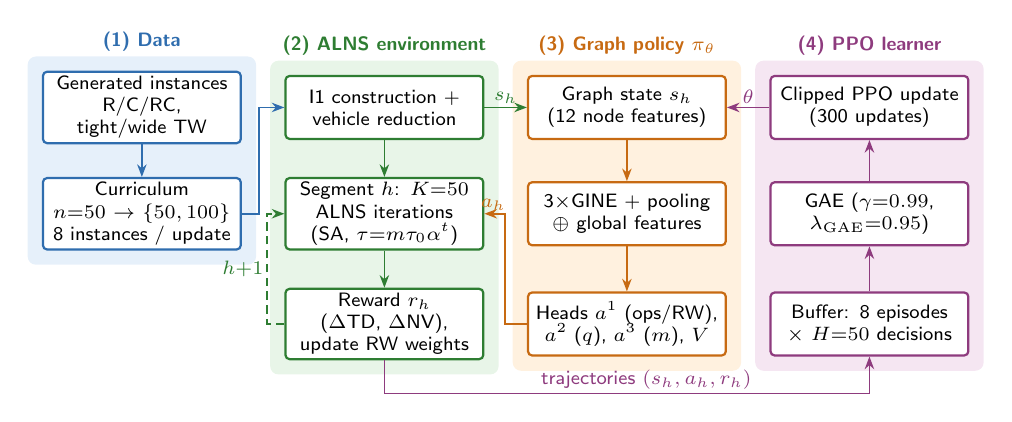
\begin{tikzpicture}[
  font=\sffamily\scriptsize,
  box/.style={draw, thick, rounded corners=1.5pt, align=center, text width=24mm, fill=white, inner sep=1.6pt, minimum height=8mm},
  arr/.style={-{Stealth[length=1.6mm]}, semithick},
  lab/.style={font=\sffamily\scriptsize, align=center, inner sep=1pt},
  ttl/.style={font=\sffamily\scriptsize\bfseries, anchor=south, inner sep=1.5pt}
]
\def\cA{0}\def\cB{3.08}\def\cC{6.16}\def\cD{9.24}
% 1 data
\node[box, draw=cDataB] (gen) at (\cA,0) {Generated instances\\ R/C/RC, tight/wide TW};
\node[box, draw=cDataB] (cur) at (\cA,-1.35) {Curriculum\\ $n{=}50\rightarrow\{50,100\}$\\ 8 instances / update};
% 2 env
\node[box, draw=cEnvB] (ini) at (\cB,0) {I1 construction +\\ vehicle reduction};
\node[box, draw=cEnvB] (seg) at (\cB,-1.35) {Segment $h$: $K{=}50$\\ ALNS iterations\\ (SA, $\tau{=}m\tau_0\alpha^t$)};
\node[box, draw=cEnvB] (rew) at (\cB,-2.75) {Reward $r_h$ ($\Delta$TD, $\Delta$NV),\\ update RW weights};
% 3 policy
\node[box, draw=cNetB] (sta) at (\cC,0) {Graph state $s_h$\\ (12 node features)};
\node[box, draw=cNetB] (enc) at (\cC,-1.35) {3$\times$GINE + pooling\\ $\oplus$ global features};
\node[box, draw=cNetB] (hed) at (\cC,-2.75) {Heads $a^1$ (ops/RW),\\ $a^2$ ($q$), $a^3$ ($m$), $V$};
% 4 PPO
\node[box, draw=cPPOB] (buf) at (\cD,-2.75) {Buffer: 8 episodes\\ $\times$ $H{=}50$ decisions};
\node[box, draw=cPPOB] (gae) at (\cD,-1.35) {GAE ($\gamma{=}0.99$,\\ $\lambda_{\mathrm{GAE}}{=}0.95$)};
\node[box, draw=cPPOB] (upd) at (\cD,0) {Clipped PPO update\\ (300 updates)};
\begin{scope}[on background layer]
\node[fill=cData, rounded corners=3pt, fit=(gen)(cur), inner sep=1.8mm] (S1) {};
\node[fill=cEnv, rounded corners=3pt, fit=(ini)(rew), inner sep=1.8mm] (S2) {};
\node[fill=cNet, rounded corners=3pt, fit=(sta)(hed), inner sep=1.8mm] (S3) {};
\node[fill=cPPO, rounded corners=3pt, fit=(upd)(buf), inner sep=1.8mm] (S4) {};
\end{scope}
\node[ttl, text=cDataB] at (S1.north) {(1) Data};
\node[ttl, text=cEnvB] at (S2.north) {(2) ALNS environment};
\node[ttl, text=cNetB] at (S3.north) {(3) Graph policy $\pi_\theta$};
\node[ttl, text=cPPOB] at (S4.north) {(4) PPO learner};
\draw[arr, cDataB] (gen) -- (cur);
\draw[arr, cEnvB] (ini) -- (seg); \draw[arr, cEnvB] (seg) -- (rew);
\draw[arr, cNetB] (sta) -- (enc); \draw[arr, cNetB] (enc) -- (hed);
\draw[arr, cPPOB] (buf) -- (gae); \draw[arr, cPPOB] (gae) -- (upd);
\draw[arr, cDataB] (cur.east) -- ++(0.22,0) |- (ini.west);
\draw[arr, cEnvB] (ini.east) -- node[lab, above]{$s_h$} (sta.west);
\draw[arr, cNetB] (hed.west) -- ++(-0.28,0) |- node[lab, pos=0.78, above]{$a_h$} (seg.east);
\draw[arr, cEnvB, densely dashed] (rew.west) -- ++(-0.22,0) |- node[lab, pos=0.25, left]{$h{+}1$} (seg.west);
\draw[arr, cPPOB] (rew.south) -- ++(0,-0.42) -| node[lab, pos=0.27, above]{trajectories $(s_h,a_h,r_h)$} ($(buf.south)$);
\draw[arr, cPPOB] (upd.west) -- node[lab, above]{$\theta$} (sta.east);
\end{tikzpicture}
\end{document}
